\chapter{چالش‌ها و محدودیت‌های محاسبات کوانتومی}
بزرگترین نکته منفی کامپیوتر کوانتومی قیمت زیاد آن است. شرکت های کوچک توانایی پرداخت هزینه این ماشین را ندارند. همچنین، در حال حاضر زیرساخت‌های ساختن کامپیوتر کوانتومی بسیار کم هستند چرا که بخش مهمی از محاسبات کوانتومی، الکترون، به راحتی توسط محیطش آسیب میبیند.
\\
تحقیقات جدید نشان داده اند که تمام کامپیوترهای کلاسیک، حتی کدهای اتمی نسبت به کامپیوترهای کوانتومی آسیب‌پذیر خواهدبود. در نتیجه باید مراقب بود که این فناوری به دست سودجویان نرسد.
\\
برای اینکه این فناوری به حداکثر ظرفیت خود برسد، باید مجموعه ای از الگوریتم‌های بدیع و مخصوص آن را پشتیبانی کنند. بدون الگوریتم های کوانتومی، کامپیوترهای کوانتومی نسبت به کامپیوترهای کلاسیک برتری‌ نخواهند داشت.
\\
چند شرکت بزرگ ادعا دارند که کامپیوتر کوانتومی ساخته‌اند. 
\verb;IBM;
و 
\verb;D Wave;
در صدر این شرکت‌ها قراردارند. اما اگر حتی کامپیوترهای کوانتومی ساخته شوند، ما از دانش استفاده موثر از آنها برخوردار نیستیم. 
\\
بخش بزرگی از مسائل توسط کامپیوترهای کلاسیک میتوانند حل شوند و استفاده از کامپیوتر کوانتومی برای آنها، منطقی نیست. کامپیوترهای کوانتومی و دانش استفاده از آنها باید تا حدی پیشرفت کند که بتوان مسائل غیرقابل حل در کامپیوترهای کلاسیک را با آنها حل کرد.
\\
کامپیوترهای کوانتومی باید در دمای بسیار پایین $460^{\circ }C$ نگهداری شوند که بسیار نزدیک به صفر مطلق است. در غیر این صورت، کارآیی نخواهند داشت.
\cite{singhbook}
\begin{figure}
\centerline{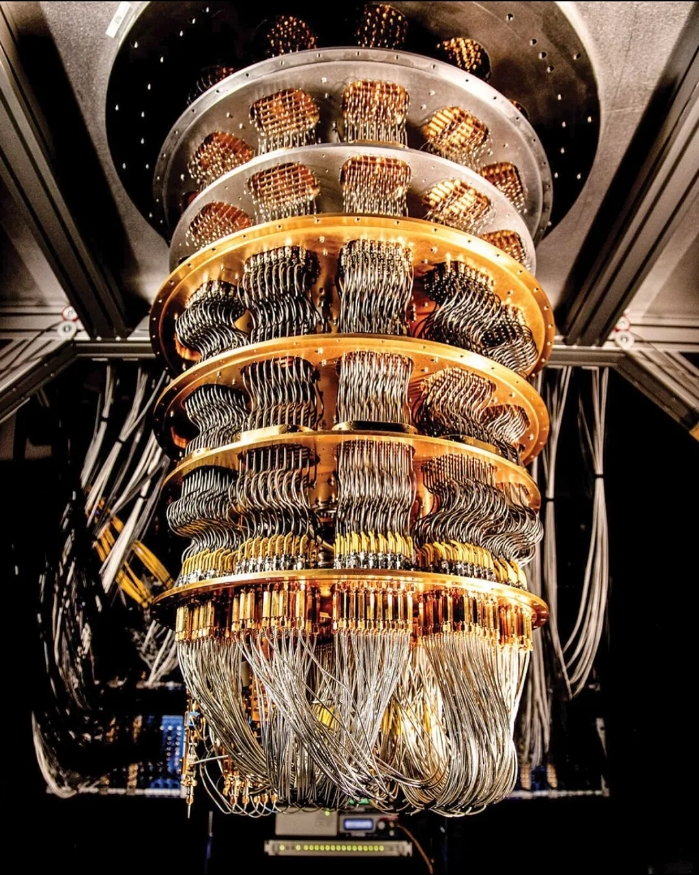
\includegraphics[width=0.6\textwidth]{computer.jpeg}}
\caption{تصویر کامپیوتر کوانتومی شرکت گوگل با ظرفیت 70 کیوبیت}
\end{figure}